% Options for packages loaded elsewhere
\PassOptionsToPackage{unicode}{hyperref}
\PassOptionsToPackage{hyphens}{url}
%
\documentclass[
  ignorenonframetext,
]{beamer}
\usepackage{pgfpages}
\setbeamertemplate{caption}[numbered]
\setbeamertemplate{caption label separator}{: }
\setbeamercolor{caption name}{fg=normal text.fg}
\beamertemplatenavigationsymbolsempty
% Prevent slide breaks in the middle of a paragraph
\widowpenalties 1 10000
\raggedbottom
\setbeamertemplate{part page}{
  \centering
  \begin{beamercolorbox}[sep=16pt,center]{part title}
    \usebeamerfont{part title}\insertpart\par
  \end{beamercolorbox}
}
\setbeamertemplate{section page}{
  \centering
  \begin{beamercolorbox}[sep=12pt,center]{part title}
    \usebeamerfont{section title}\insertsection\par
  \end{beamercolorbox}
}
\setbeamertemplate{subsection page}{
  \centering
  \begin{beamercolorbox}[sep=8pt,center]{part title}
    \usebeamerfont{subsection title}\insertsubsection\par
  \end{beamercolorbox}
}
\AtBeginPart{
  \frame{\partpage}
}
\AtBeginSection{
  \ifbibliography
  \else
    \frame{\sectionpage}
  \fi
}
\AtBeginSubsection{
  \frame{\subsectionpage}
}

\usepackage{amsmath,amssymb}
\usepackage{lmodern}
\usepackage{iftex}
\ifPDFTeX
  \usepackage[T1]{fontenc}
  \usepackage[utf8]{inputenc}
  \usepackage{textcomp} % provide euro and other symbols
\else % if luatex or xetex
  \usepackage{unicode-math}
  \defaultfontfeatures{Scale=MatchLowercase}
  \defaultfontfeatures[\rmfamily]{Ligatures=TeX,Scale=1}
\fi
% Use upquote if available, for straight quotes in verbatim environments
\IfFileExists{upquote.sty}{\usepackage{upquote}}{}
\IfFileExists{microtype.sty}{% use microtype if available
  \usepackage[]{microtype}
  \UseMicrotypeSet[protrusion]{basicmath} % disable protrusion for tt fonts
}{}
\makeatletter
\@ifundefined{KOMAClassName}{% if non-KOMA class
  \IfFileExists{parskip.sty}{%
    \usepackage{parskip}
  }{% else
    \setlength{\parindent}{0pt}
    \setlength{\parskip}{6pt plus 2pt minus 1pt}}
}{% if KOMA class
  \KOMAoptions{parskip=half}}
\makeatother
\usepackage{xcolor}
\newif\ifbibliography
\setlength{\emergencystretch}{3em} % prevent overfull lines
\setcounter{secnumdepth}{-\maxdimen} % remove section numbering


\providecommand{\tightlist}{%
  \setlength{\itemsep}{0pt}\setlength{\parskip}{0pt}}\usepackage{longtable,booktabs,array}
\usepackage{calc} % for calculating minipage widths
\usepackage{caption}
% Make caption package work with longtable
\makeatletter
\def\fnum@table{\tablename~\thetable}
\makeatother
\usepackage{graphicx}
\makeatletter
\def\maxwidth{\ifdim\Gin@nat@width>\linewidth\linewidth\else\Gin@nat@width\fi}
\def\maxheight{\ifdim\Gin@nat@height>\textheight\textheight\else\Gin@nat@height\fi}
\makeatother
% Scale images if necessary, so that they will not overflow the page
% margins by default, and it is still possible to overwrite the defaults
% using explicit options in \includegraphics[width, height, ...]{}
\setkeys{Gin}{width=\maxwidth,height=\maxheight,keepaspectratio}
% Set default figure placement to htbp
\makeatletter
\def\fps@figure{htbp}
\makeatother

\makeatletter
\makeatother
\makeatletter
\makeatother
\makeatletter
\@ifpackageloaded{caption}{}{\usepackage{caption}}
\AtBeginDocument{%
\ifdefined\contentsname
  \renewcommand*\contentsname{Table of contents}
\else
  \newcommand\contentsname{Table of contents}
\fi
\ifdefined\listfigurename
  \renewcommand*\listfigurename{List of Figures}
\else
  \newcommand\listfigurename{List of Figures}
\fi
\ifdefined\listtablename
  \renewcommand*\listtablename{List of Tables}
\else
  \newcommand\listtablename{List of Tables}
\fi
\ifdefined\figurename
  \renewcommand*\figurename{Figure}
\else
  \newcommand\figurename{Figure}
\fi
\ifdefined\tablename
  \renewcommand*\tablename{Table}
\else
  \newcommand\tablename{Table}
\fi
}
\@ifpackageloaded{float}{}{\usepackage{float}}
\floatstyle{ruled}
\@ifundefined{c@chapter}{\newfloat{codelisting}{h}{lop}}{\newfloat{codelisting}{h}{lop}[chapter]}
\floatname{codelisting}{Listing}
\newcommand*\listoflistings{\listof{codelisting}{List of Listings}}
\makeatother
\makeatletter
\@ifpackageloaded{caption}{}{\usepackage{caption}}
\@ifpackageloaded{subcaption}{}{\usepackage{subcaption}}
\makeatother
\makeatletter
\@ifpackageloaded{tcolorbox}{}{\usepackage[many]{tcolorbox}}
\makeatother
\makeatletter
\@ifundefined{shadecolor}{\definecolor{shadecolor}{rgb}{.97, .97, .97}}
\makeatother
\makeatletter
\makeatother
\ifLuaTeX
  \usepackage{selnolig}  % disable illegal ligatures
\fi
\IfFileExists{bookmark.sty}{\usepackage{bookmark}}{\usepackage{hyperref}}
\IfFileExists{xurl.sty}{\usepackage{xurl}}{} % add URL line breaks if available
\urlstyle{same} % disable monospaced font for URLs
\hypersetup{
  pdfauthor={Ryan Teo},
  hidelinks,
  pdfcreator={LaTeX via pandoc}}

\author{Ryan Teo}
\date{2022-07-19}

\begin{document}
\ifdefined\Shaded\renewenvironment{Shaded}{\begin{tcolorbox}[sharp corners, boxrule=0pt, interior hidden, enhanced, breakable, frame hidden, borderline west={3pt}{0pt}{shadecolor}]}{\end{tcolorbox}}\fi

\begin{frame}{Action items from previous meeting}
\protect\hypertarget{action-items-from-previous-meeting}{}
\begin{enumerate}
\tightlist
\item
  Visualise extra-long delays
\item
  Analyse test-specific case data
\end{enumerate}
\end{frame}

\begin{frame}{Extra-long delays}
\protect\hypertarget{extra-long-delays}{}
\begin{figure}

{\centering 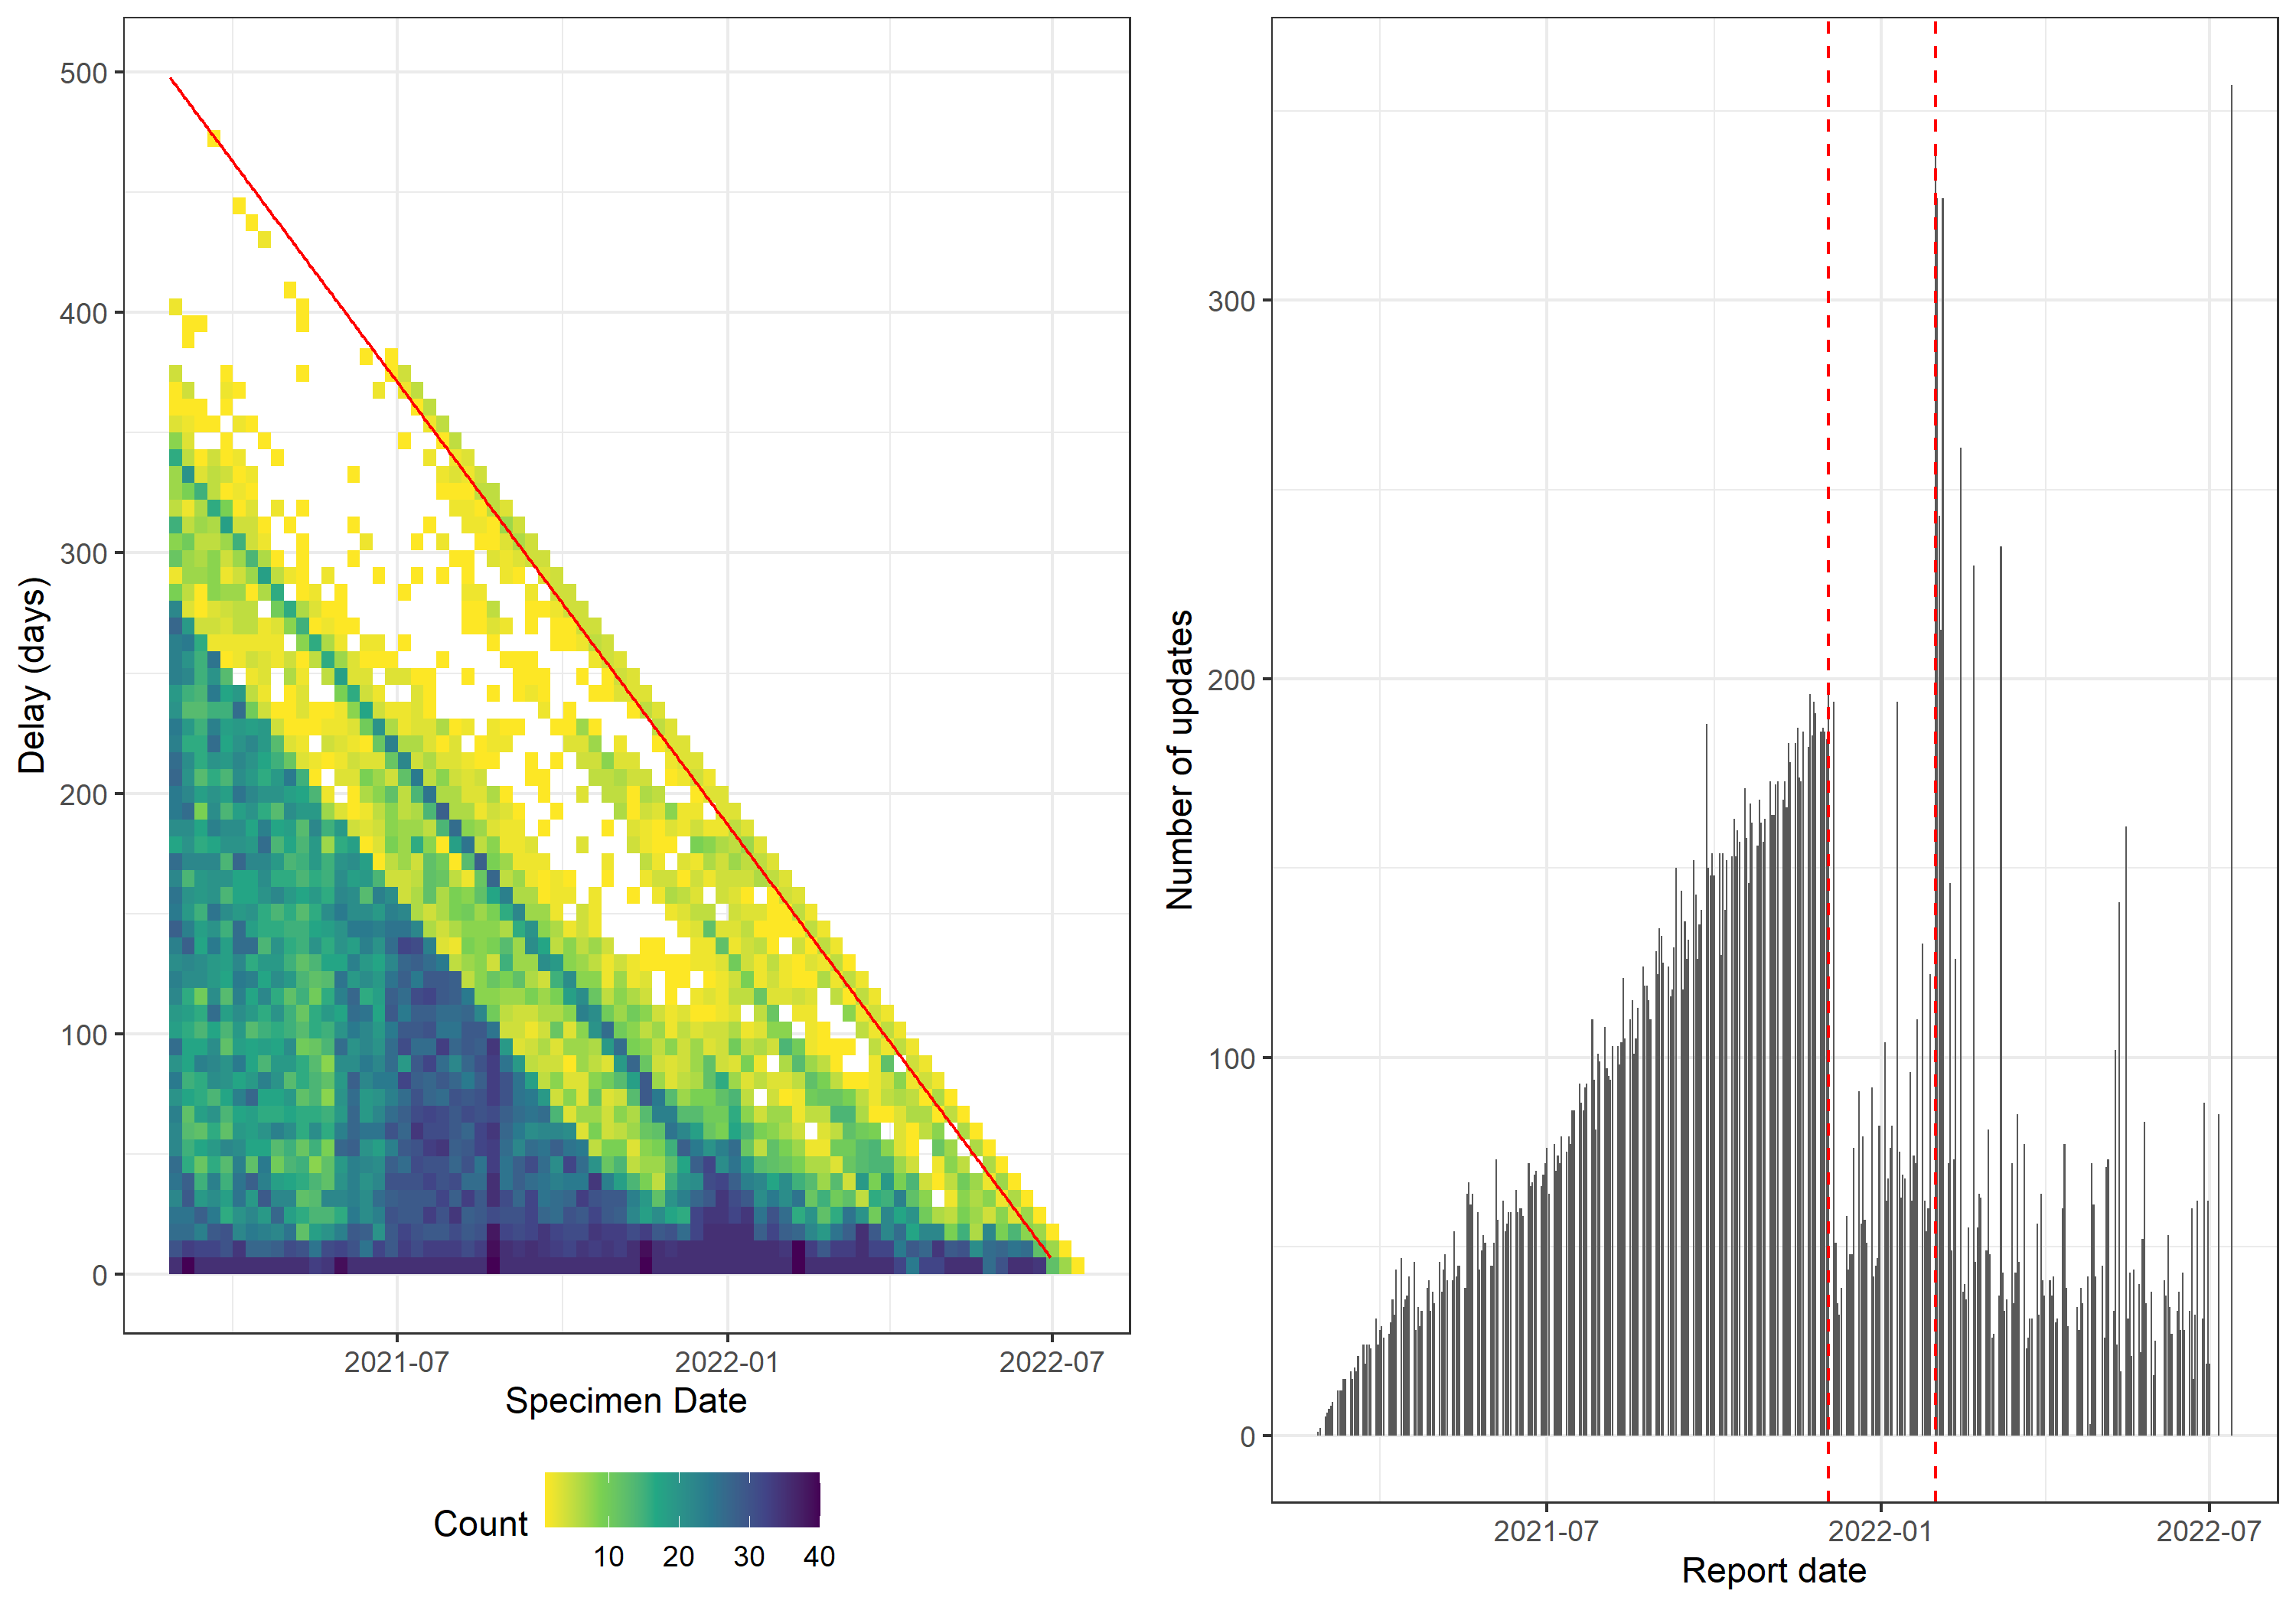
\includegraphics{progress_presentation_files/figure-beamer/unnamed-chunk-2-1.png}

}

\end{figure}
\end{frame}

\begin{frame}{Extra-long delays}
\protect\hypertarget{extra-long-delays-1}{}
\begin{itemize}
\tightlist
\item
  Number of updates per report date increased quite steadily till
  03/12/21

  \begin{itemize}
  \tightlist
  \item
    Unsure about why this happened
  \end{itemize}
\item
  Large number of updates on 31/1/22

  \begin{itemize}
  \tightlist
  \item
    \href{https://coronavirus.data.gov.uk/details/whats-new/record/beb802ac-1ed2-47ac-b314-69a5c3f712b5}{Updating
    of case definition} to include multiple infection episodes
  \item
    Cases by specimen date revised back to the beginning of the pandemic
  \end{itemize}
\item
  Conclusion: might be reasonable to assume a maximum delay of
  \textasciitilde50 days?
\end{itemize}
\end{frame}

\begin{frame}{Distribution of cases by delay}
\protect\hypertarget{distribution-of-cases-by-delay}{}
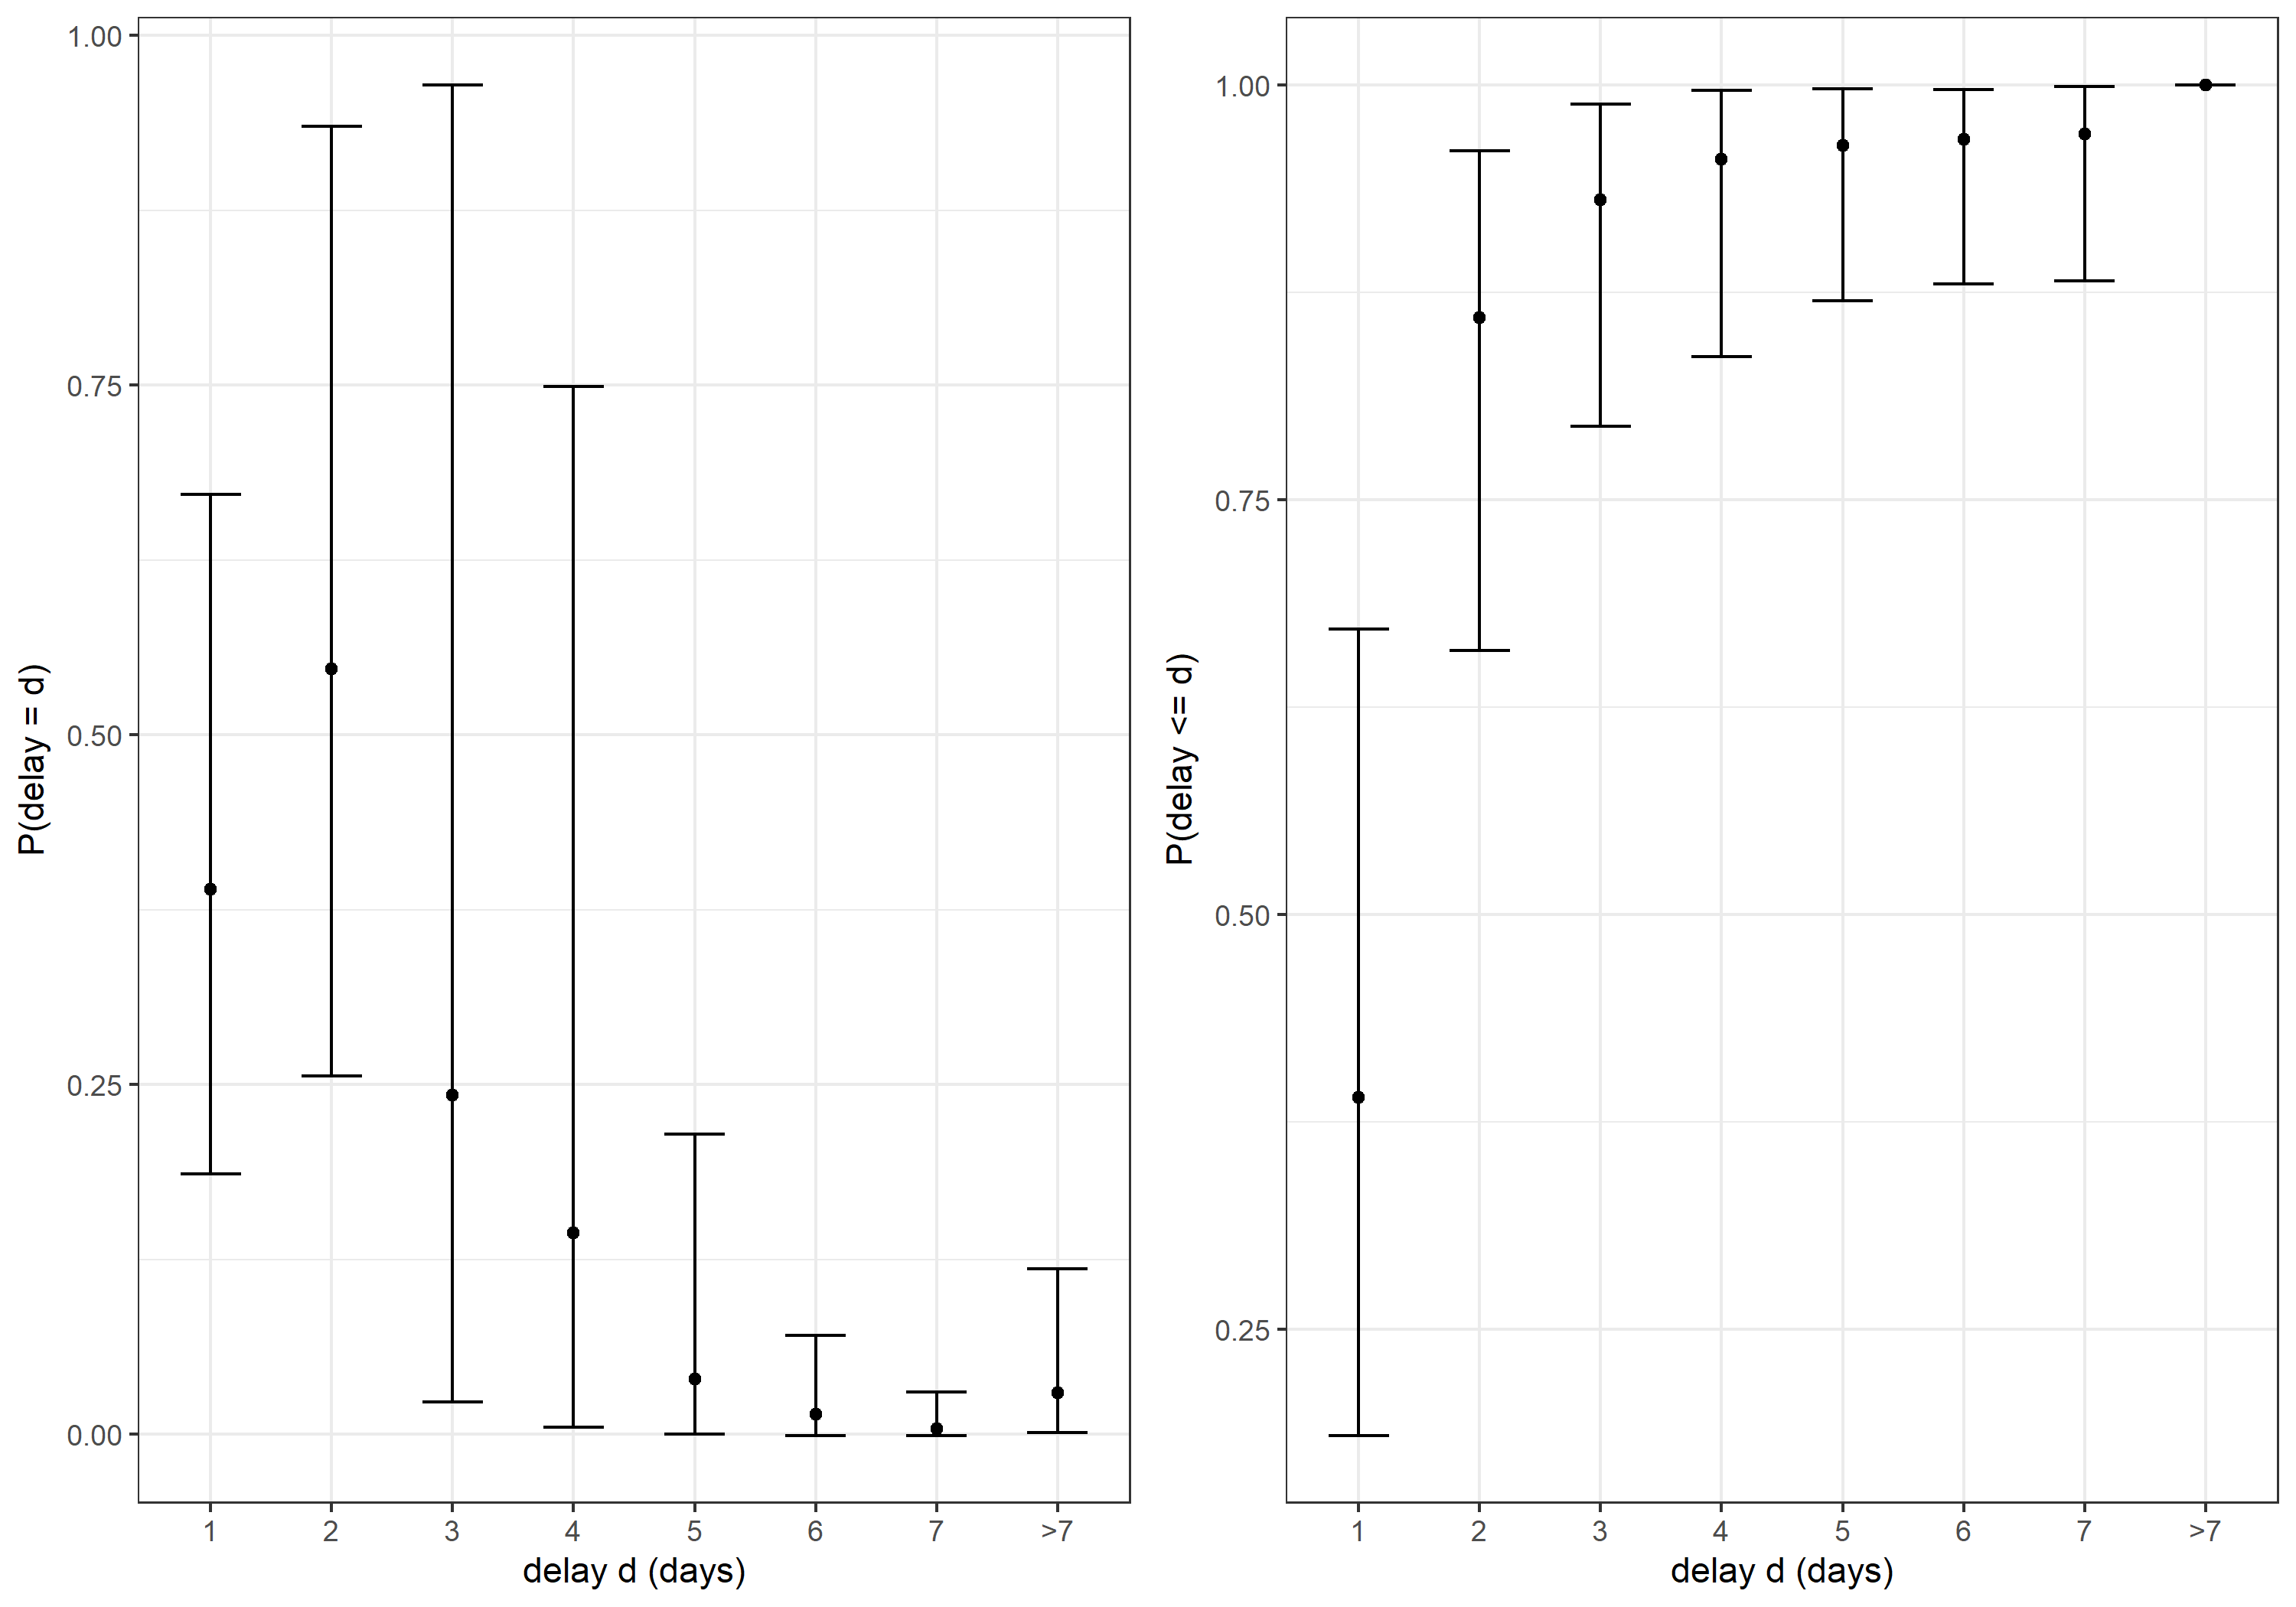
\includegraphics{progress_presentation_files/figure-beamer/unnamed-chunk-3-1.png}
\end{frame}

\begin{frame}{Day of week}
\protect\hypertarget{day-of-week}{}
\emph{Sanity check}

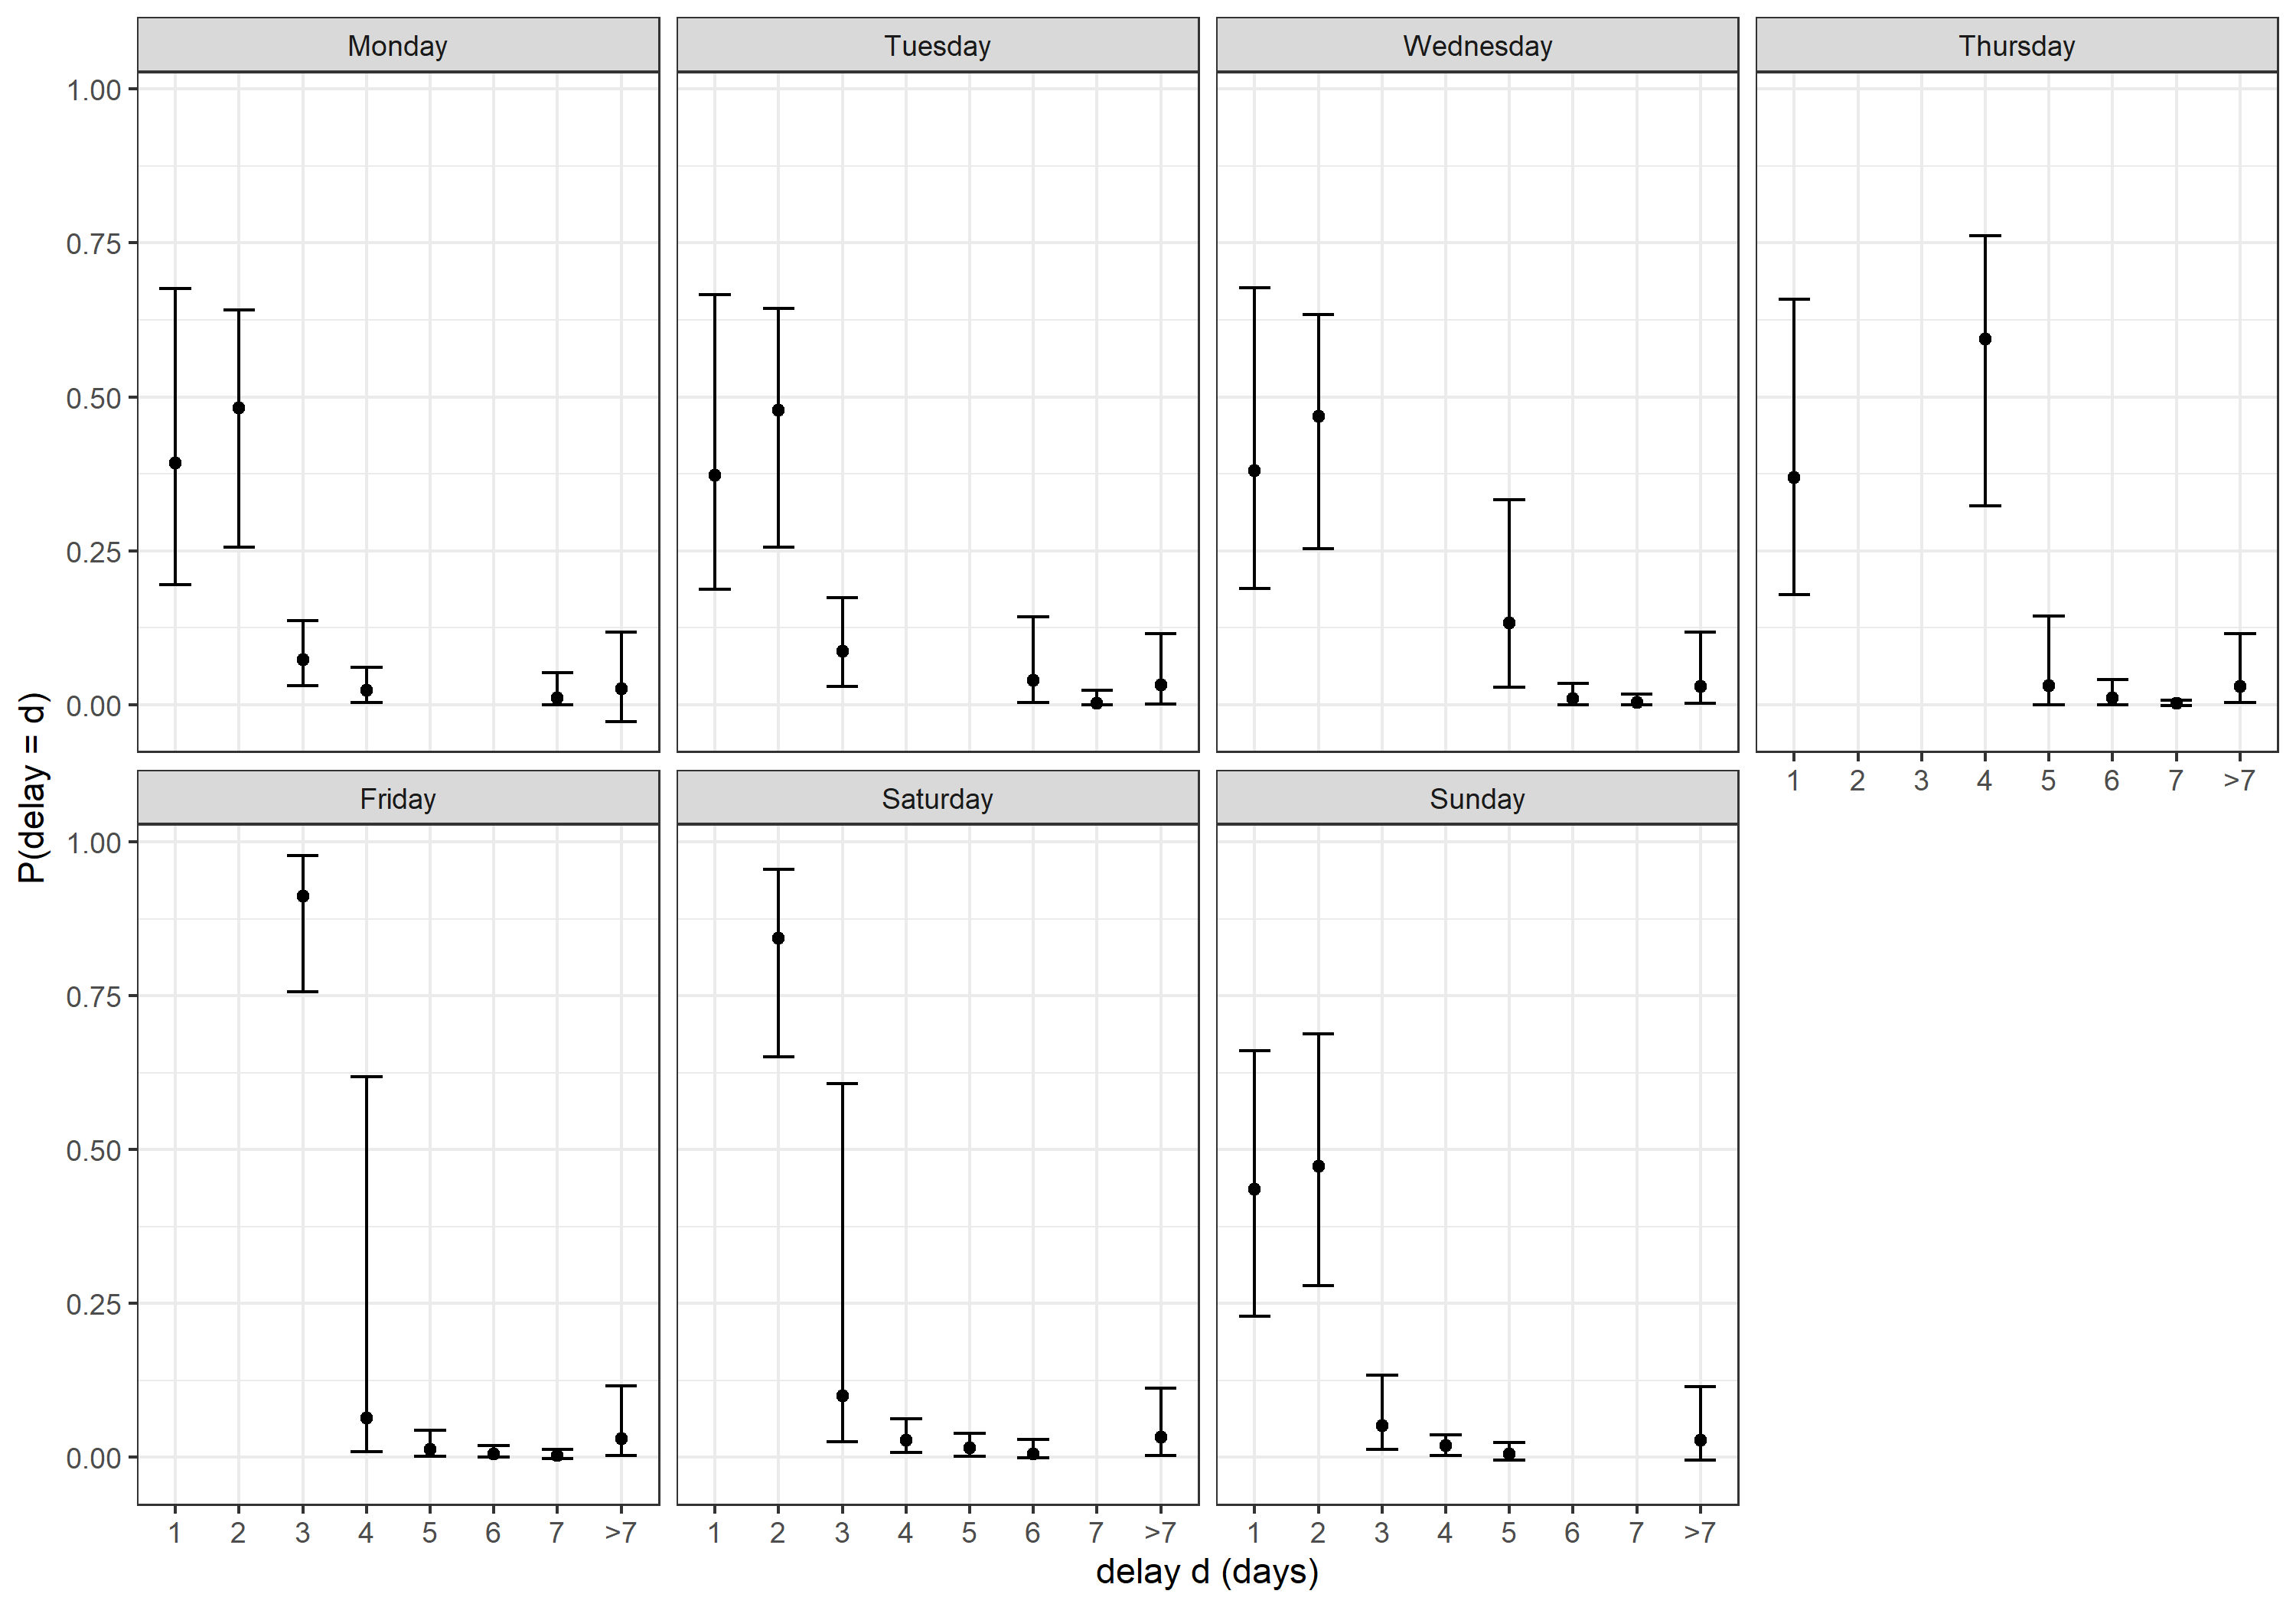
\includegraphics{progress_presentation_files/figure-beamer/unnamed-chunk-4-1.png}
\end{frame}

\begin{frame}[fragile]{Test-specific case data}
\protect\hypertarget{test-specific-case-data}{}
\texttt{New\ cases\ by\ specimen\ date} is the sum of three separate
data sources:

\begin{enumerate}
\tightlist
\item
  LFD confirmed by PCR

  \begin{itemize}
  \tightlist
  \item
    Identified by LFD and confirmed by PCR within 3 days
  \item
    Date reflects LFD test date\\
  \end{itemize}
\item
  LFD only

  \begin{itemize}
  \tightlist
  \item
    Identified by LFD and not confirmed by PCR within 3 days
  \item
    If subsequent PCR is negative, cases will be removed
  \end{itemize}
\item
  PCR only

  \begin{itemize}
  \tightlist
  \item
    Identified by PCR excluding those identified by LFD within 3 days
  \end{itemize}
\end{enumerate}
\end{frame}

\begin{frame}{Test type}
\protect\hypertarget{test-type}{}
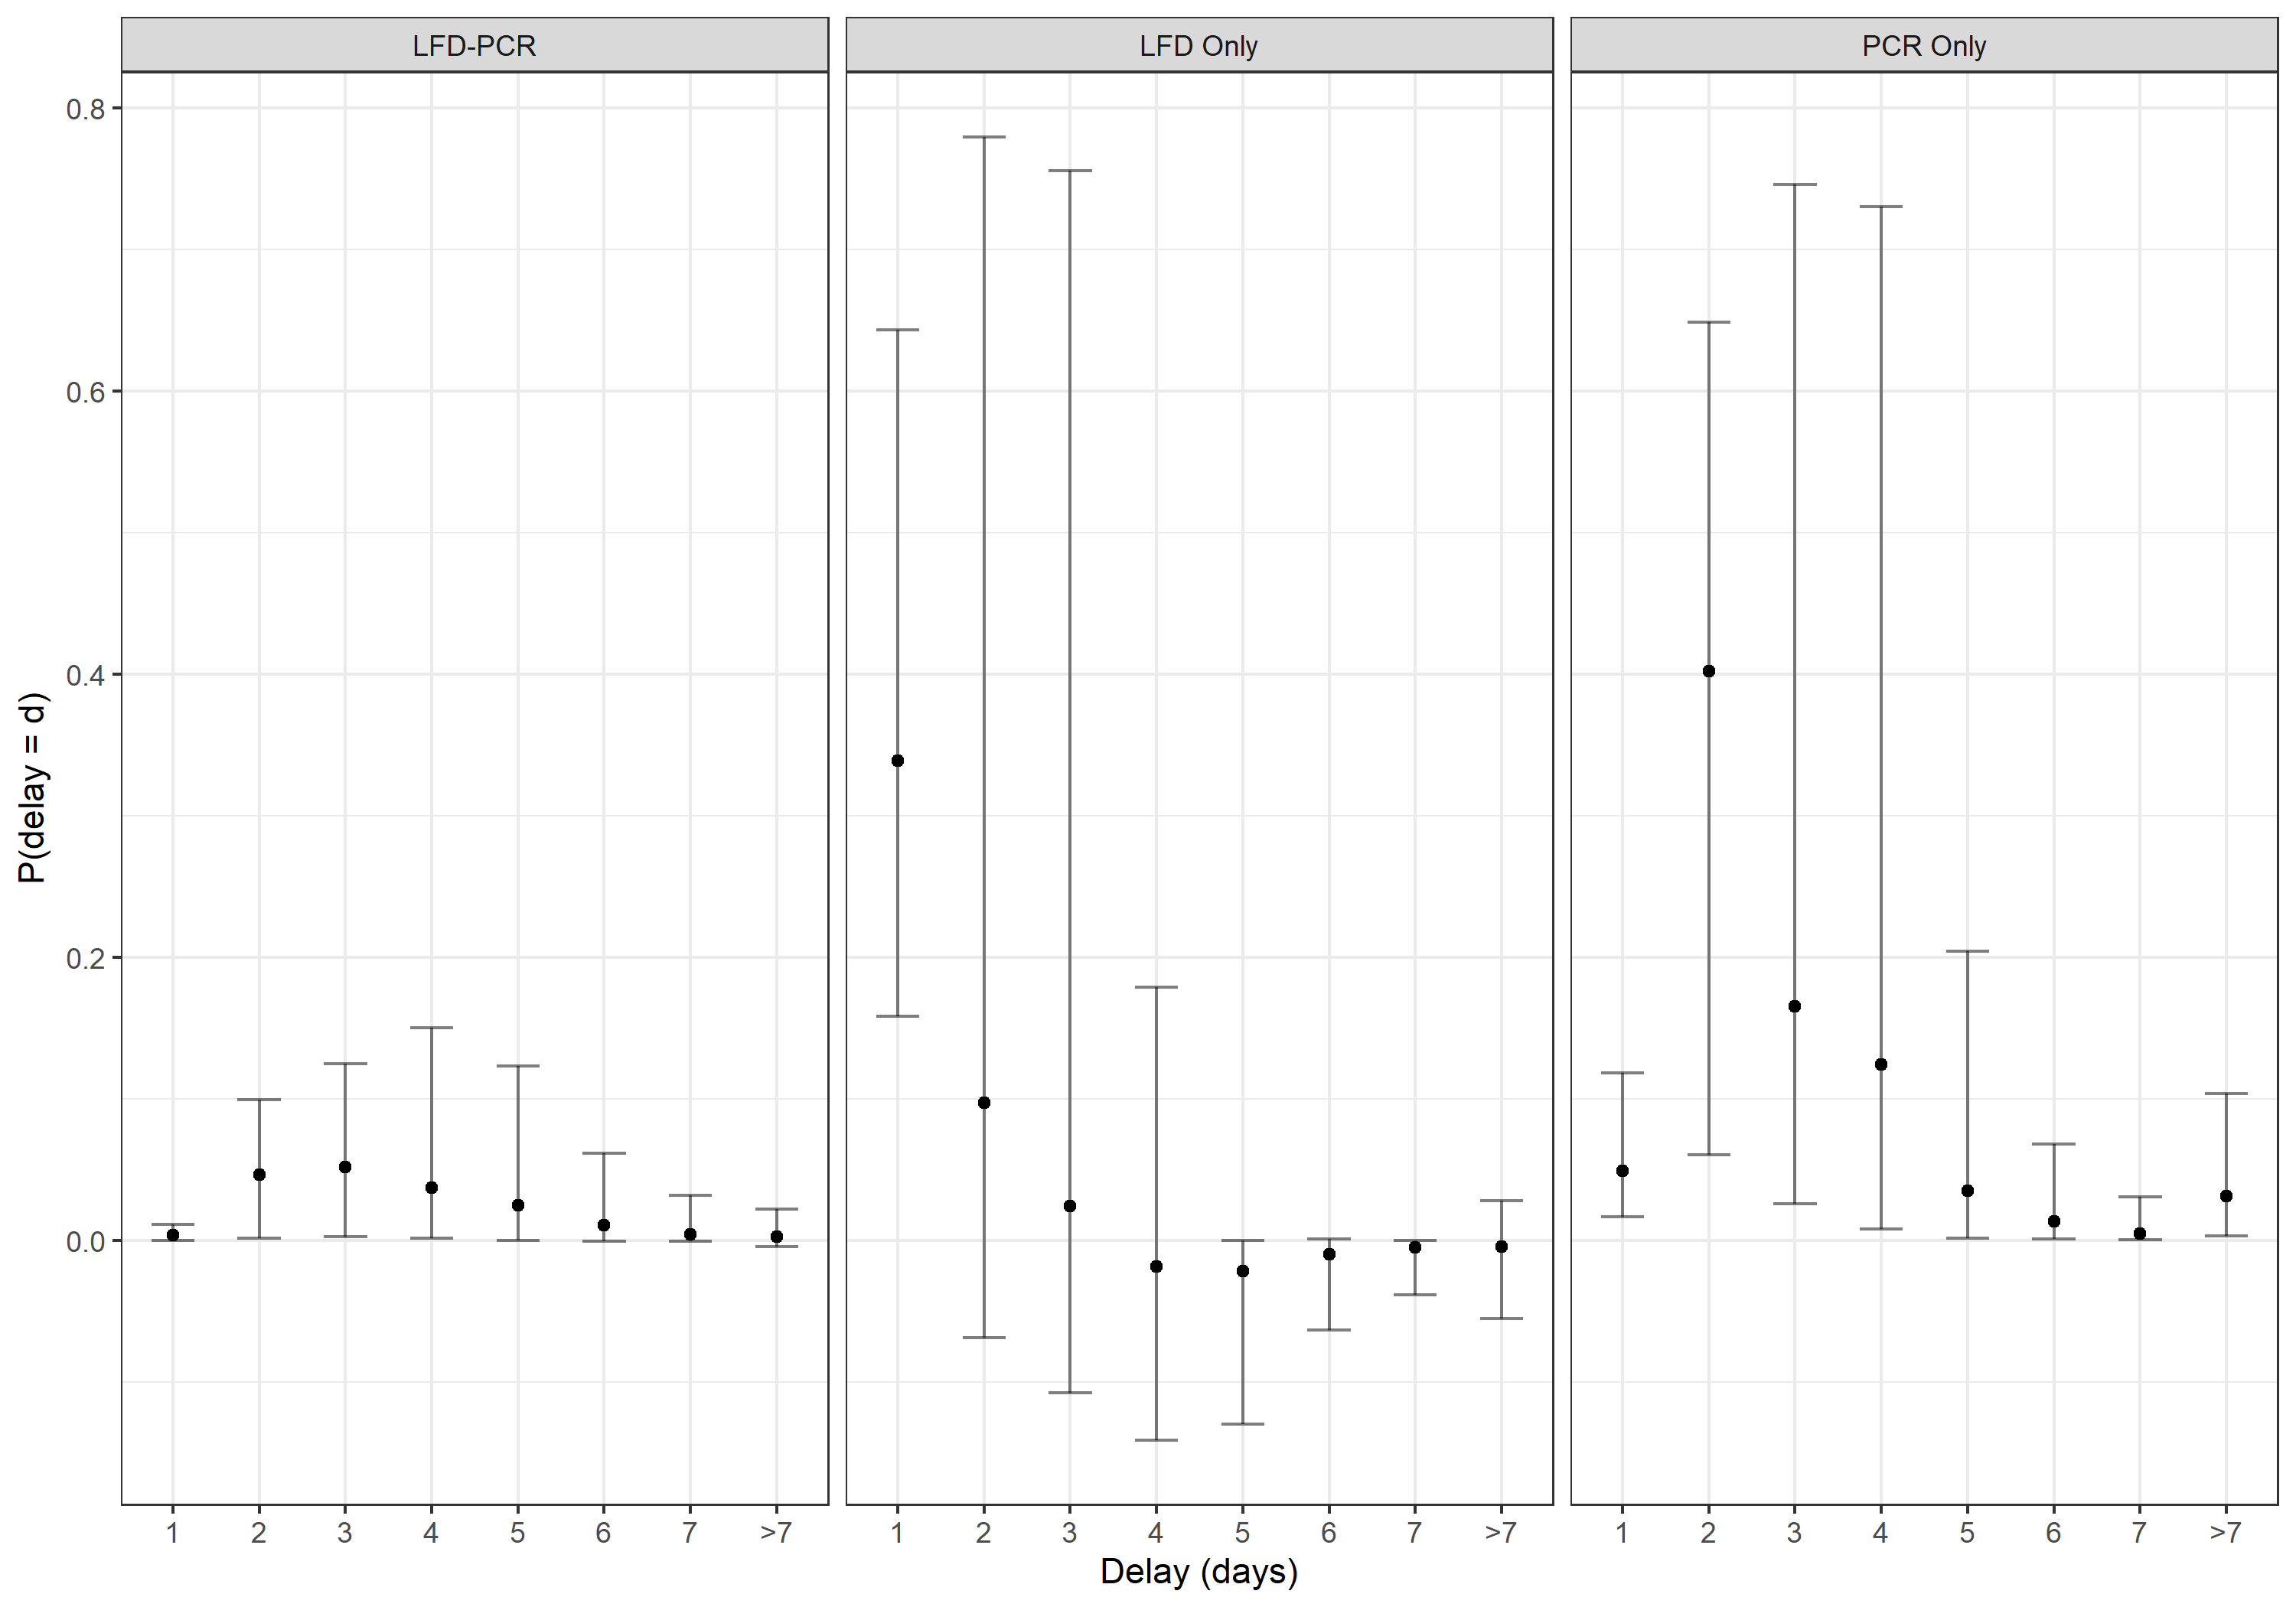
\includegraphics{progress_presentation_files/figure-beamer/unnamed-chunk-5-1.png}
\end{frame}

\begin{frame}{Test type}
\protect\hypertarget{test-type-1}{}
\begin{itemize}
\tightlist
\item
  Might be able to nowcast LFD-PCR and PCR only streams separately

  \begin{itemize}
  \tightlist
  \item
    updates for these streams are not all positive, occasionally some
    case definition revisions lead to large negative updates
  \item
    e.g.~\href{https://coronavirus.data.gov.uk/details/whats-new/record/8055ae4e-ba2a-450a-bff8-42e9e4d1575b}{Revision
    to episode-based case definition} on 1/2/22 led to large drops in
    PCR only cases for a few dates (7-10/1/22) in the thousands
  \end{itemize}
\item
  Need a different model for LFD only stream
\end{itemize}
\end{frame}

\begin{frame}[fragile]{Next steps}
\protect\hypertarget{next-steps}{}
\begin{itemize}
\tightlist
\item
  Try out \texttt{epinowcast}
\item
  Explore further stratification by location and age
\item
  Create counterfactual datasets with alternative reporting schedule
  (weekdaily vs weekly)
\end{itemize}
\end{frame}



\end{document}
